Next, we should install the .NET SDK (unexpectedly again) in order to run our application.
Proceeding, we refer to the Microsoft documentation article named
\href{https://docs.microsoft.com/en-us/dotnet/core/install/linux-ubuntu}
{\texttt{Install the .NET SDK or the .NET Runtime on Ubuntu}}~\cite{MSDN_Ubuntu}, precisely the version is 20.04.
As per documentation, consider the following commands to install .NET 6.0 SDK to your Ubuntu VM
\begin{figure}[H]
    \centering
    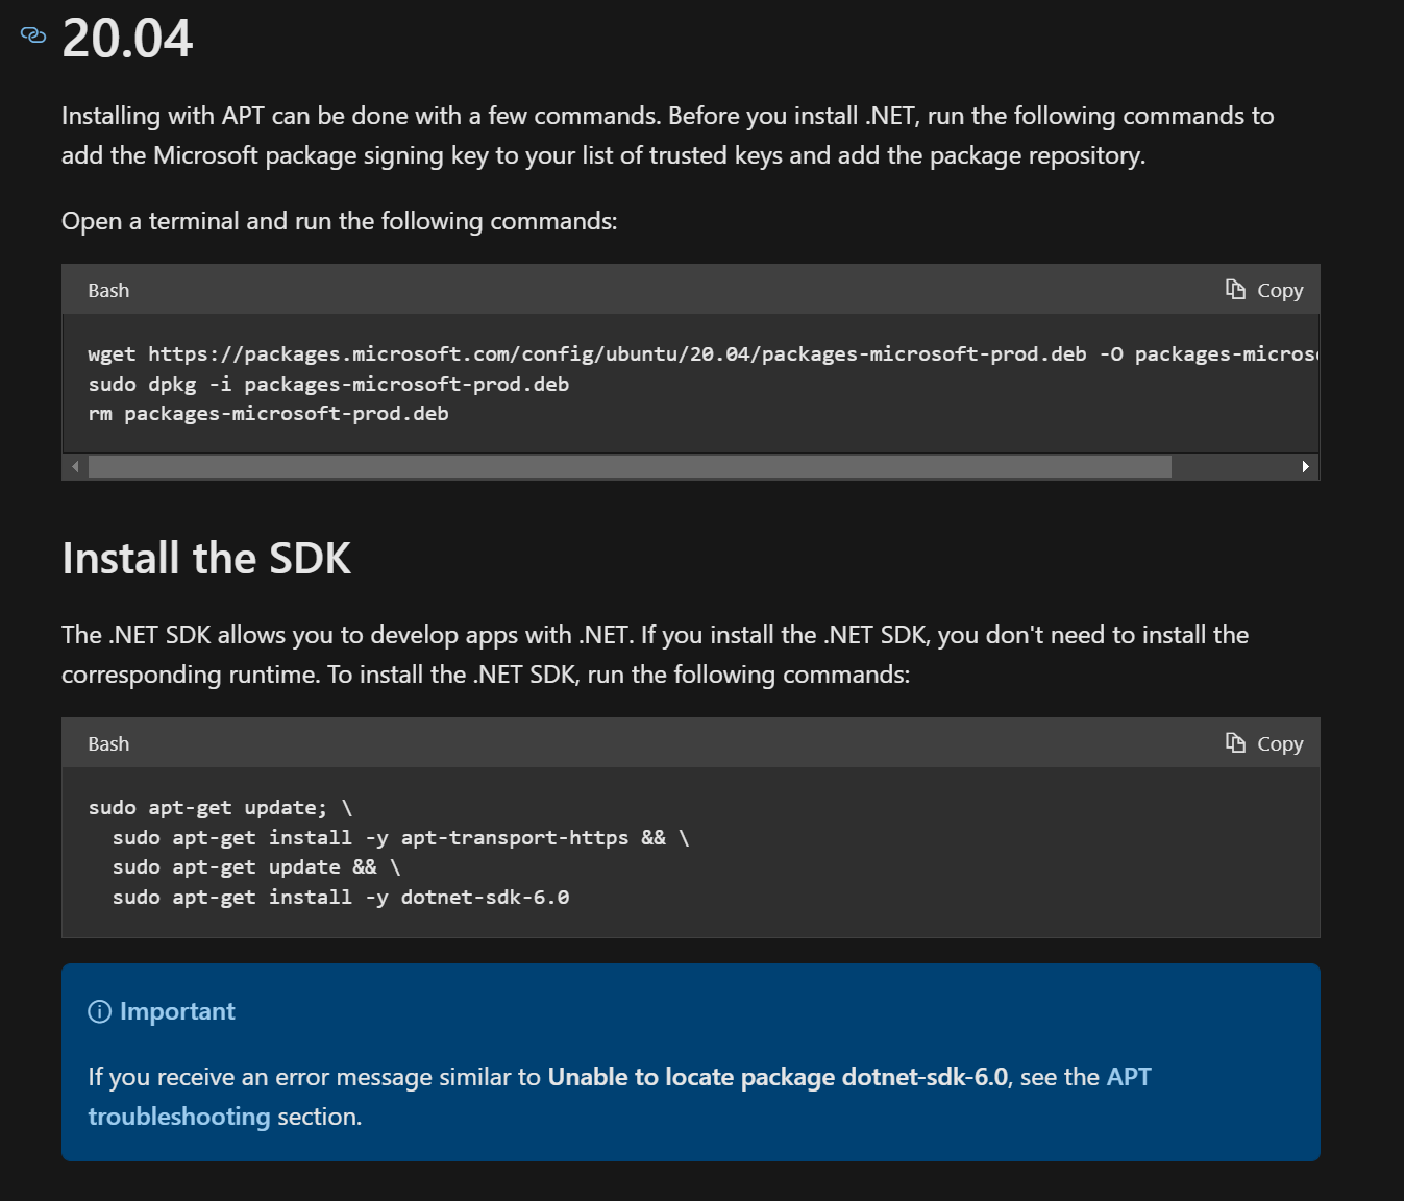
\includegraphics[width=1\textwidth]{img/03_1_sdk_documentation}
    ~\caption{Ubuntu 20.04 install .NET 6.0 SDK MSDN.}\label{fig:figure2}
\end{figure}
Prepare your virtual machine applying the commands
\begin{itemize}
    \item \texttt{wget https://packages.microsoft.com/config/ubuntu/20.04/packages-microsoft-prod.deb -O packages-microsoft-prod.deb}
    \item \texttt{sudo dpkg -i packages-microsoft-prod.deb}
    \item \texttt{rm packages-microsoft-prod.deb}
\end{itemize}
The terminal output is as follows
\begin{figure}[H]
    \centering
    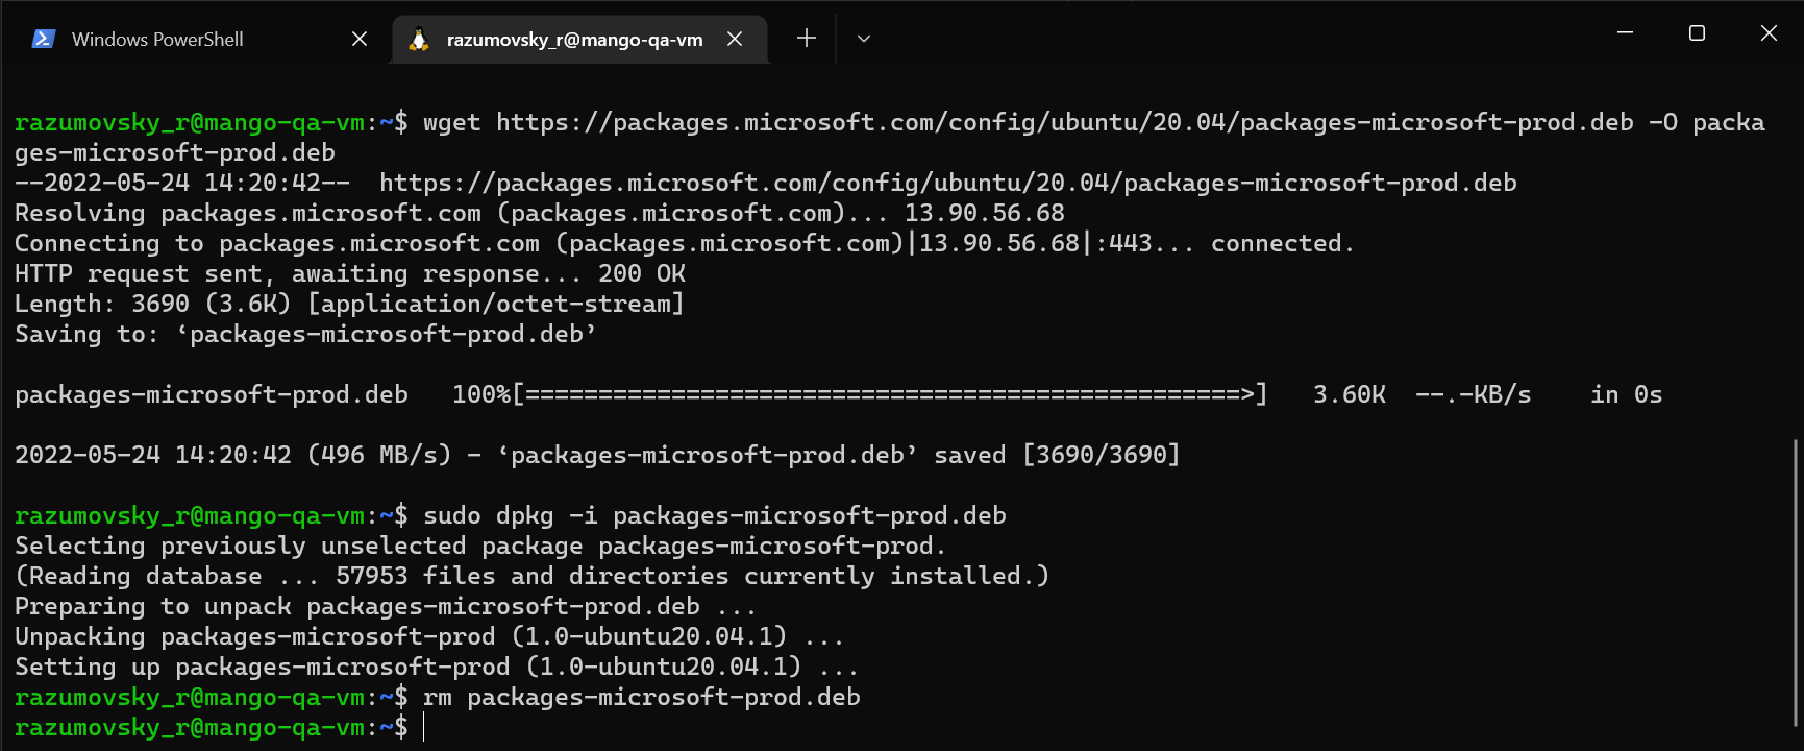
\includegraphics[width=1\textwidth]{img/03_3_vm_prepare}
    ~\caption{Virtual machine preparation..}\label{fig:figure3}
\end{figure}
Apply the following commands in order to install the SDK
\begin{itemize}
    \item \texttt{sudo apt-get update}
    \item \texttt{sudo apt-get install -y apt-transport-https}
    \item \texttt{sudo apt-get update}
    \item \texttt{sudo apt-get install -y dotnet-sdk-6.0}
\end{itemize}
The terminal output after .NET 6.0 SDK installation is as follows
\begin{figure}[H]
    \centering
    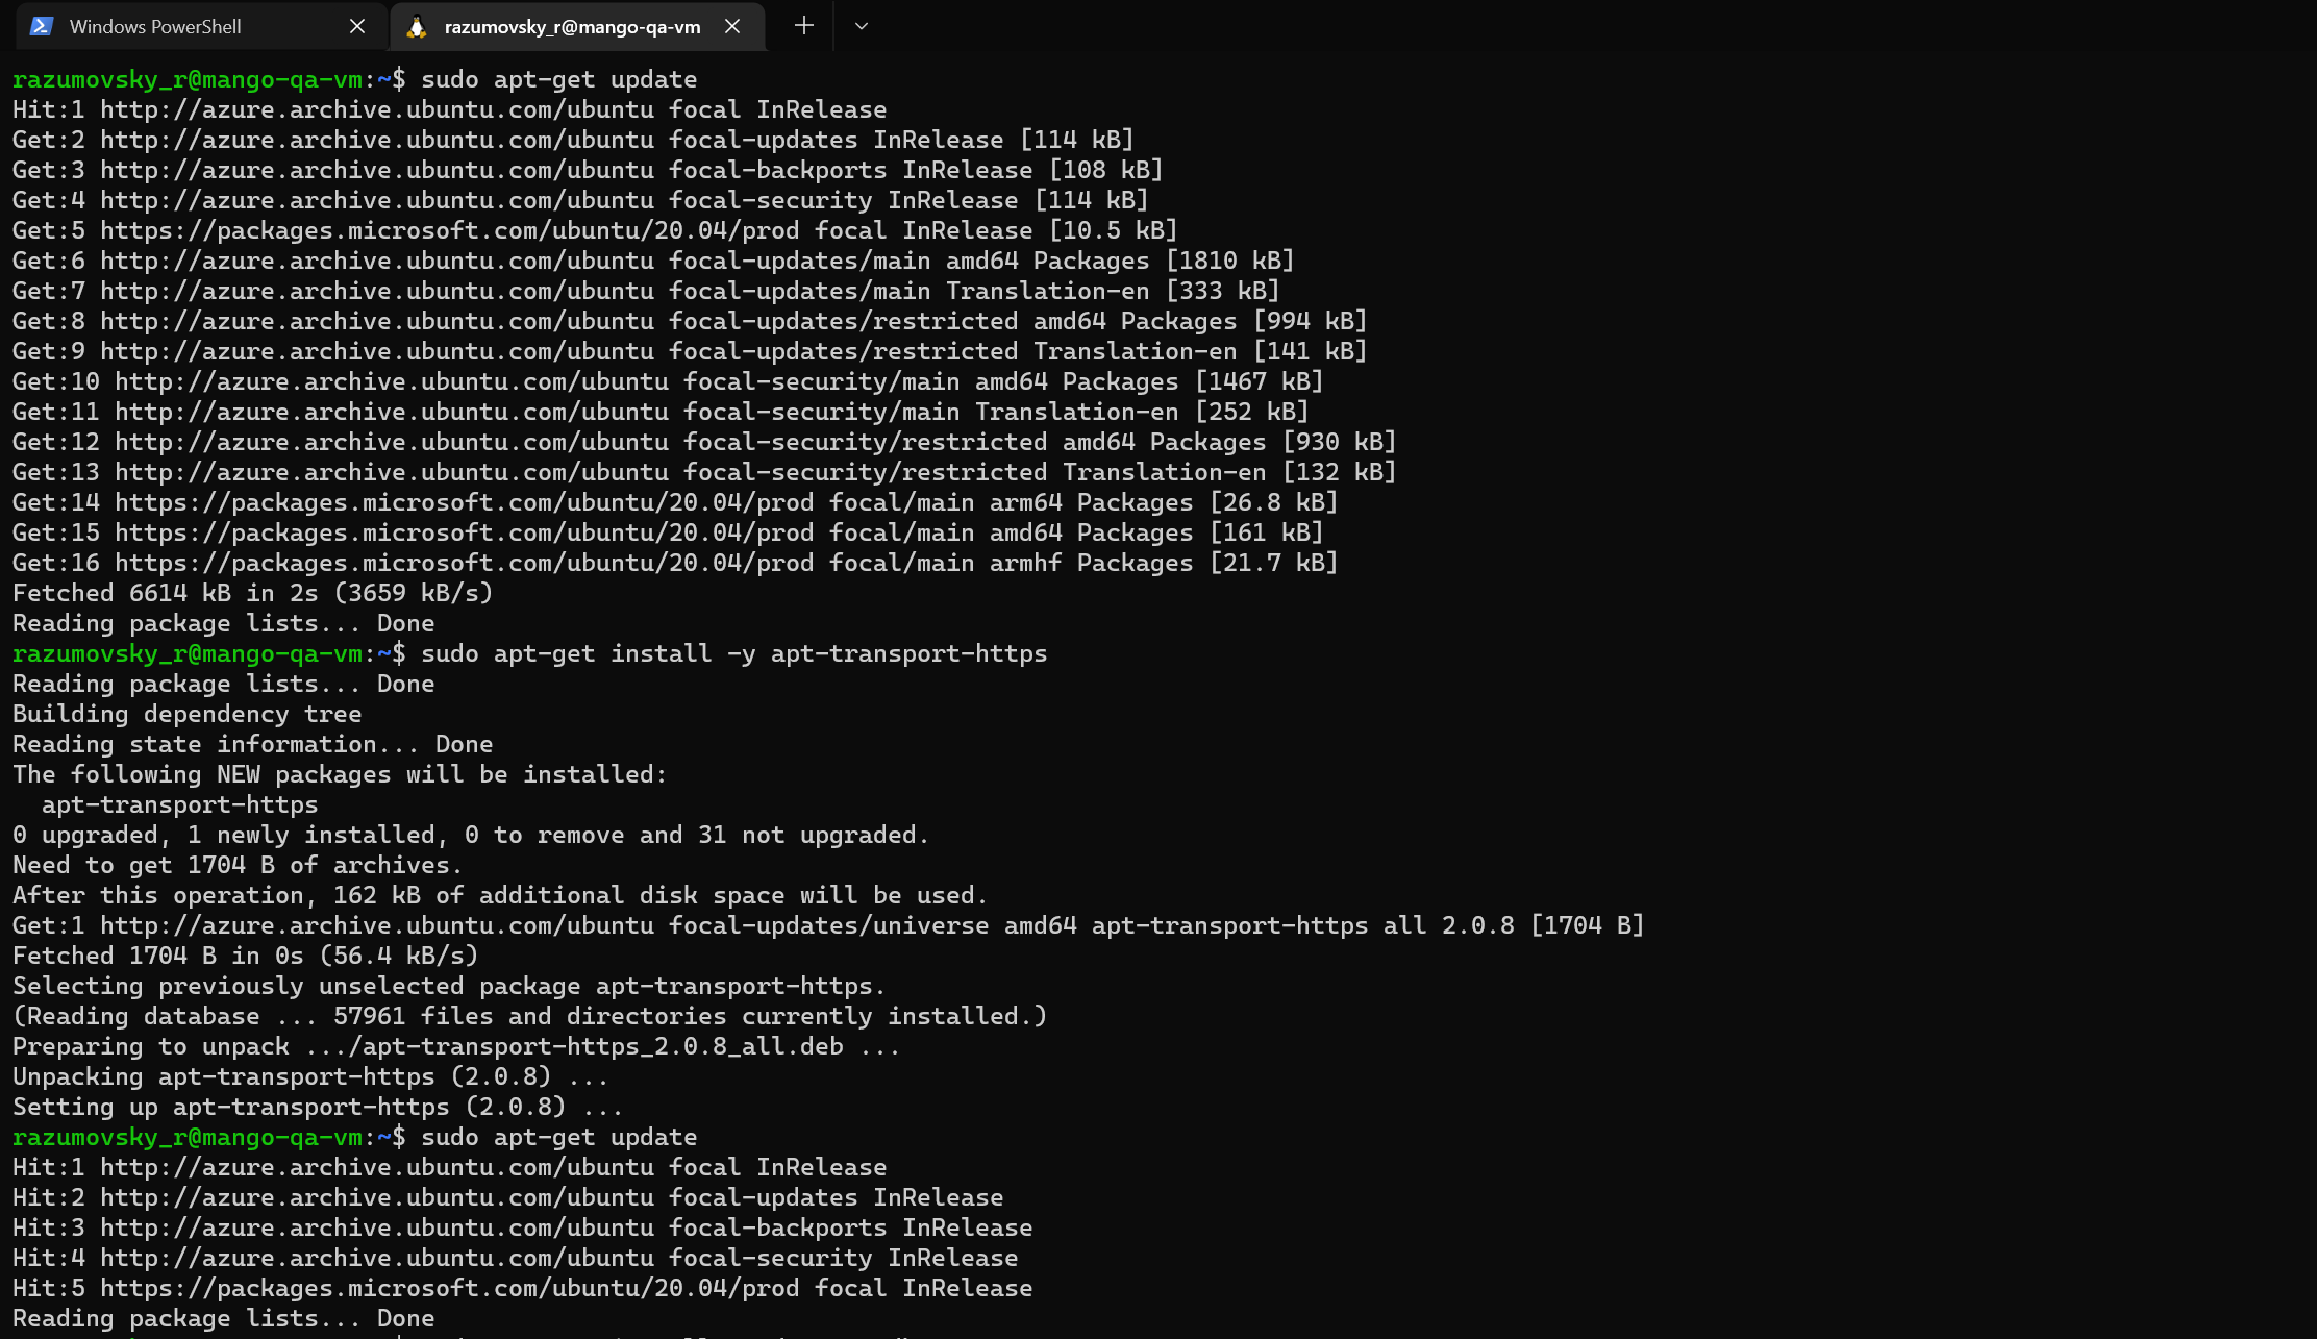
\includegraphics[width=1\textwidth]{img/03_4_sdk_install_1}
    ~\caption{Ubuntu 20.04 install .NET 6.0 SDK terminal output.}\label{fig:figure4}
\end{figure}
\begin{figure}[H]
    \centering
    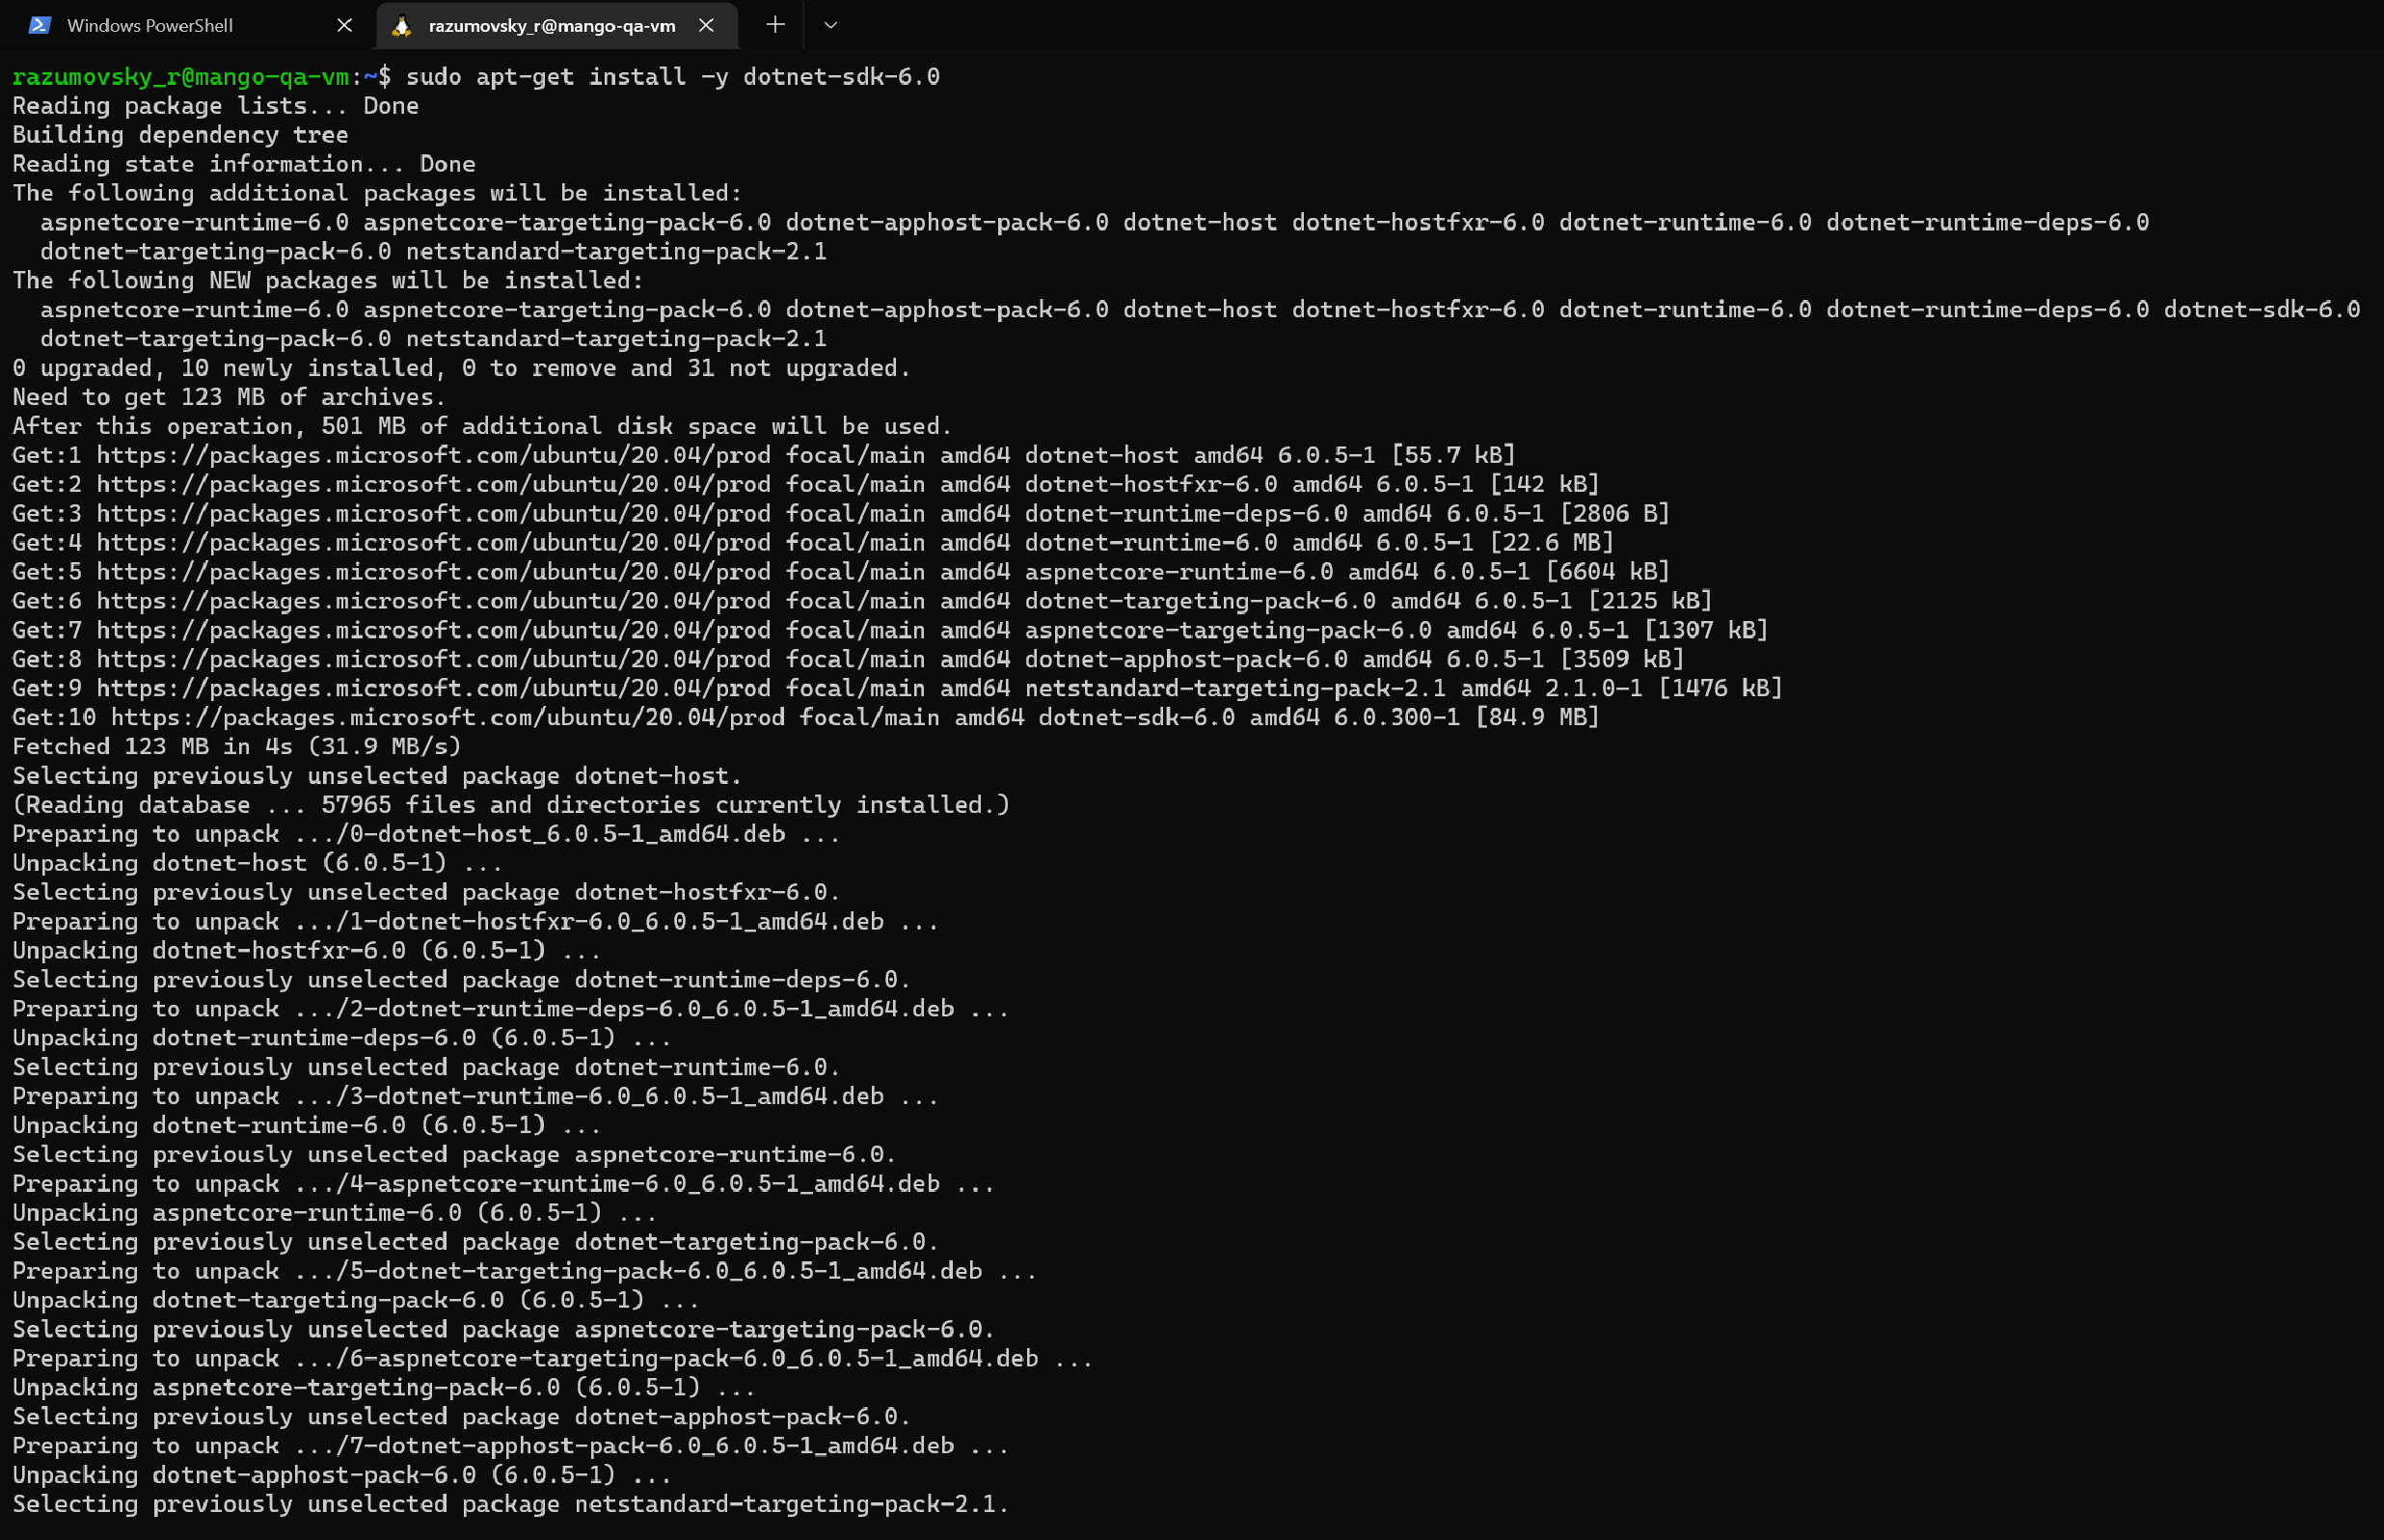
\includegraphics[width=1\textwidth]{img/03_4_sdk_install_2}
    ~\caption{Ubuntu 20.04 install .NET 6.0 SDK terminal output.}\label{fig:figure5}
\end{figure}
\begin{figure}[H]
    \centering
    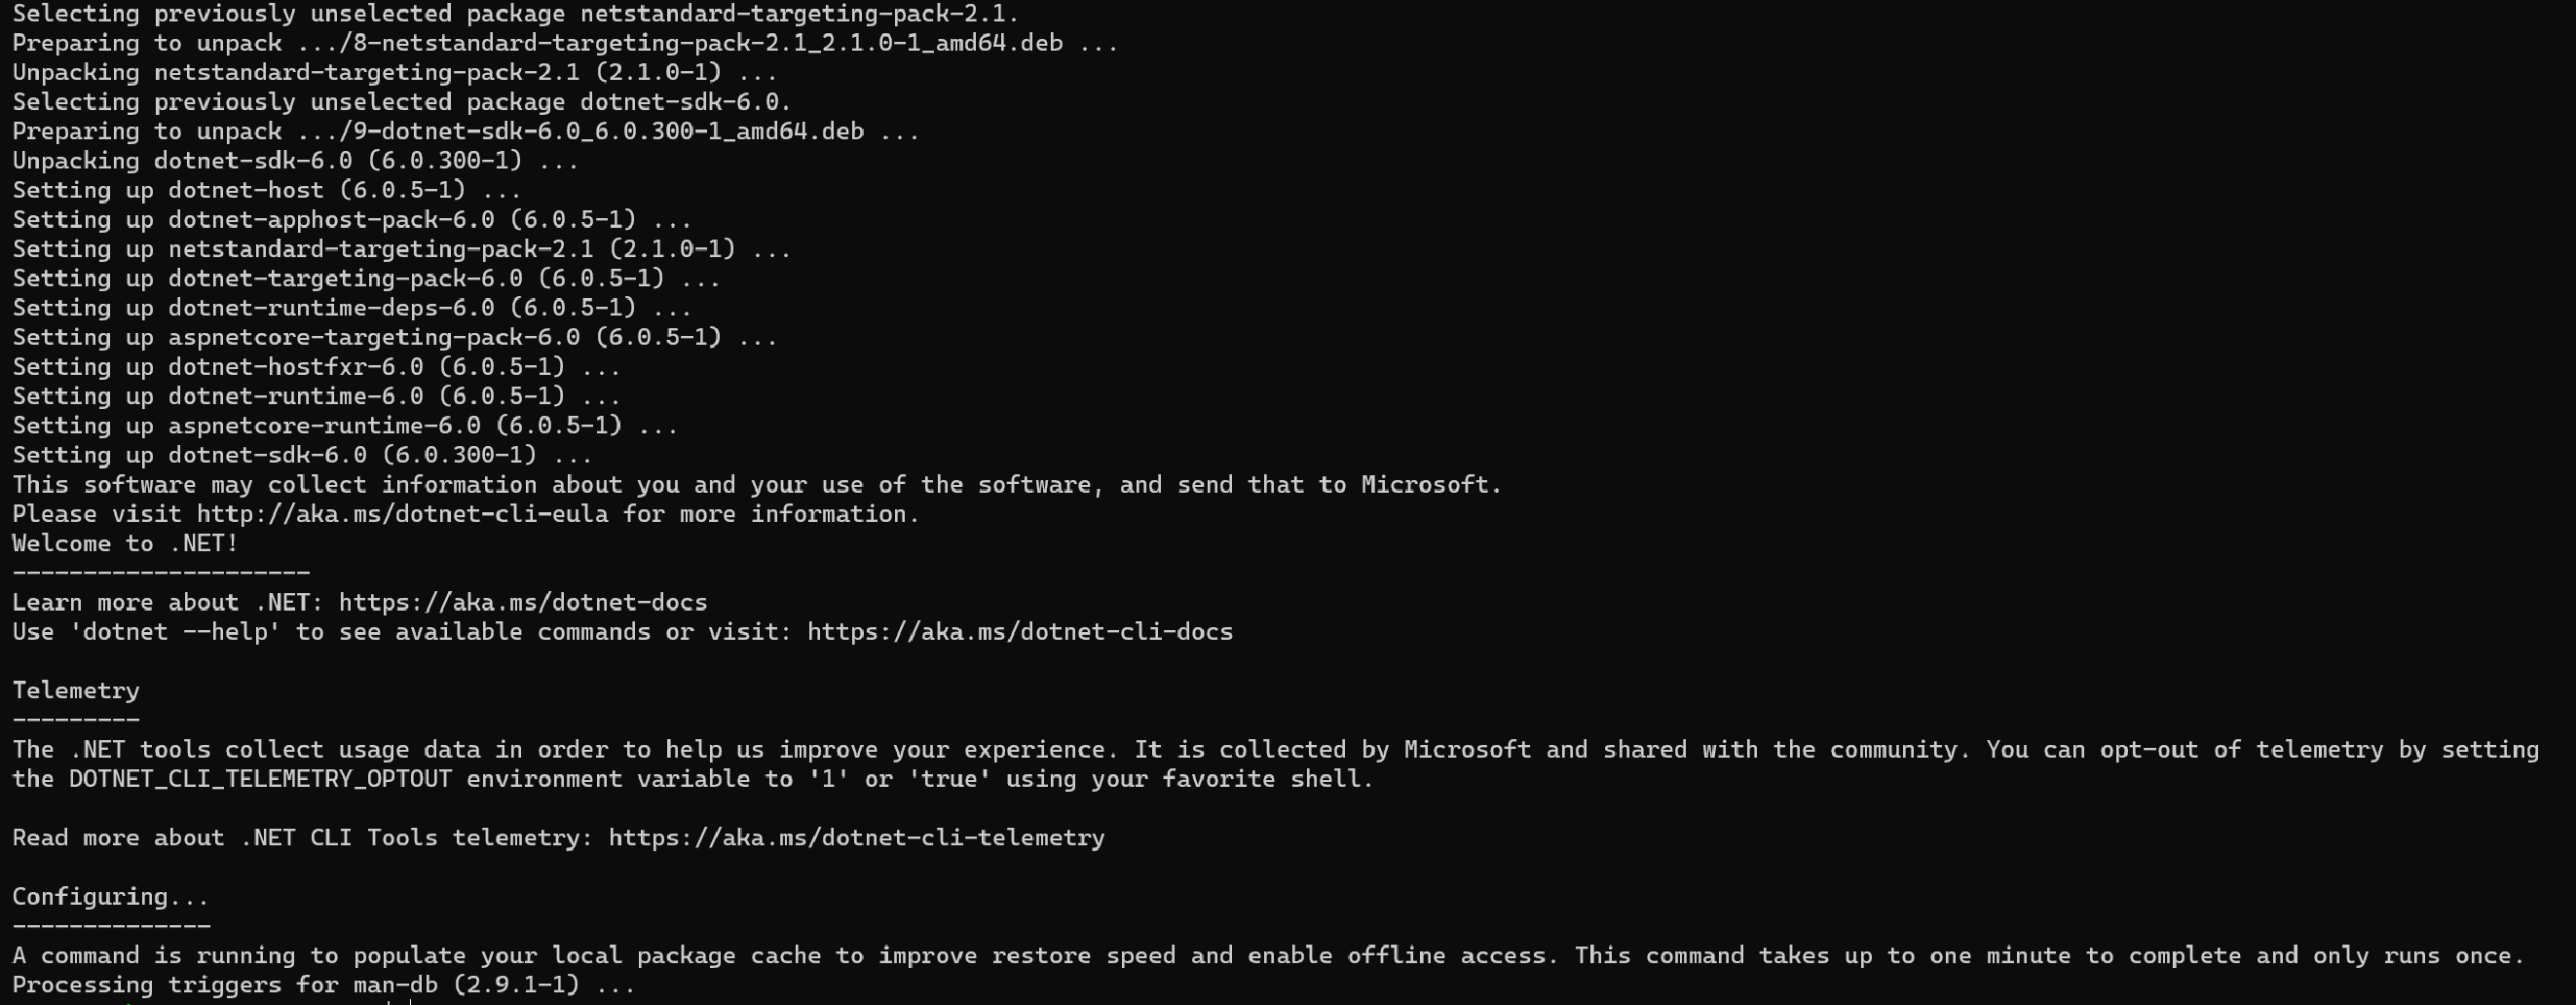
\includegraphics[width=1\textwidth]{img/03_4_sdk_install_3}
    ~\caption{Ubuntu 20.04 install .NET 6.0 SDK terminal output.}\label{fig:figure6}
\end{figure}

In order to install the .NET Runtime we refer again to the Microsoft documentation, that is
\begin{figure}[H]
    \centering
    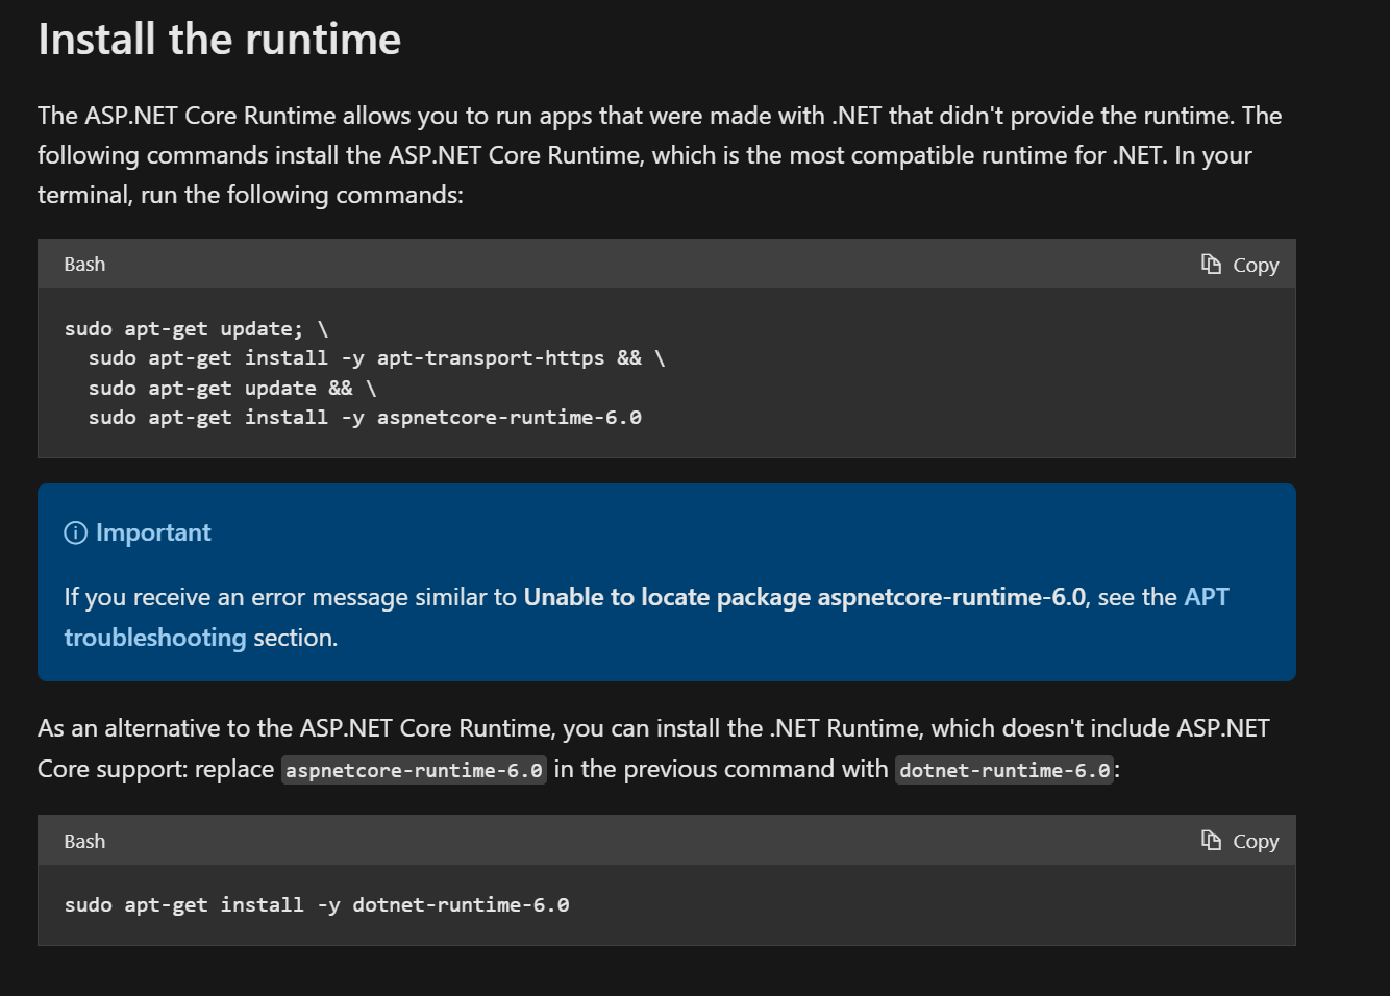
\includegraphics[width=1\textwidth]{img/03_2_runtime_documentation}
    ~\caption{Install the .NET SDK or the .NET Runtime on Ubuntu MSDN.}\label{fig:figure7}
\end{figure}
We install .NET runtime using the commands
\begin{itemize}
    \item \texttt{sudo apt-get update}
    \item \texttt{sudo apt-get install -y apt-transport-https}
    \item \texttt{sudo apt-get update}
    \item \texttt{sudo apt-get install -y aspnetcore-runtime-6.0}
\end{itemize}
Terminal output as follows
\begin{figure}[H]
    \centering
    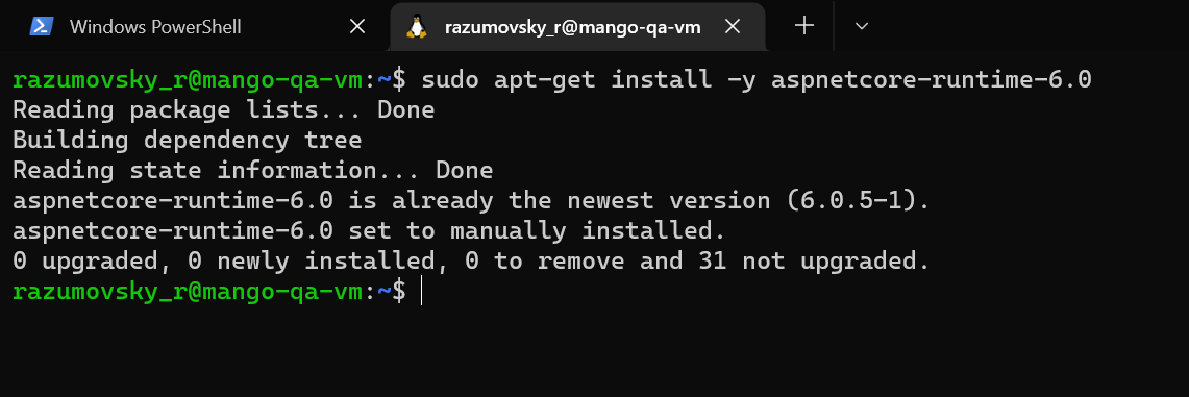
\includegraphics[width=1\textwidth]{img/03_6_runtime_install}
    ~\caption{Ubuntu 20.04 install .NET 6.0 Runtime terminal output.}\label{fig:figure8}
\end{figure}
Therefore, the .NET SDK and Runtime are installed so that we are able to run specified .NET app on behalf of
our Ubuntu virtual machine.
